\usepackage{amsmath,amssymb}
\usepackage{amsthm}


\usepackage{tikz}
\usepackage[francais]{babel}
\usepackage{pgfplots}
\usepackage{pgfplotstable}
\usepackage{subcaption}
% \newlist{longenumerate}{enumerate}{4}
% \setlist[longenumerate,0]{label=\usebeamerfont*{enumerate item}%
%   \usebeamercolor[fg]{enumerate item}
%   \usebeamertemplate{enumerate item}}
%  
\usepgflibrary{shapes.geometric}
\usetikzlibrary{fit}
\usetikzlibrary{backgrounds}
\usetikzlibrary{positioning} 
%\usetikzlibrary{pgfplots.external}
%\usetikzlibrary{pgfplots.units} 
%\usepgfplotslibrary{external}
\usetikzlibrary{shapes.multipart}
\usetikzlibrary{fit}

\newtheorem{property}{Property}

\newcommand{\vect}[1]{ {\boldsymbol {#1}}}
\newcommand{\eye}{1}
\newcommand{\kron}{\bigotimes}

 \beamerdefaultoverlayspecification{}
\setbeamercovered{transparent}

\newenvironment{plusenv}{\alt{\setbeamertemplate{itemize item}{$\textcolor{green}{\oplus}$}}
{\setbeamertemplate{itemize item}{$\textcolor{gray}{\oplus}$}}}{}
\newenvironment{moinsenv}{\alt{\setbeamertemplate{itemize item}{$\textcolor{red}{\ominus}$}}
{\setbeamertemplate{itemize item}{$\textcolor{gray}{\ominus}$}}}{}
\def\plusitem{\item<+-| plus@+-| handout:plus@0-> }
\def\moinsitem{\item<+-| moins@+-| handout:moins@0-> }

\newenvironment{pmenv}{\alt{\setbeamertemplate{itemize item}{$\textcolor{blue}{\pm}$}}
{\setbeamertemplate{itemize item}{$\textcolor{gray}{\pm}$}}}{}
\def\pmitem{\item<+-| pm@+-| handout:pm@0-> }

\setbeamercolor{section in toc}{fg=red}
\setbeamercolor{section in toc shaded}{fg=blue}

\setbeamercolor{subsection in toc}{fg=red}
\setbeamercolor{subsection in toc shaded}{fg=blue}

\pgfplotsset{compat=1.6}

\title[Navier-Stokes]{Simulation du Jet D'Eau de A à Y:\\ Algorithme numérique pour résoudre les équations de Navier-Stokes incompressible}


\author{Pablo Strasser}


\institute[Unige] % (optional, but mostly needed)
{University of Geneva}



\date[\today] % (optional, should be abbreviation of conference name)
{\today}

\subject{Navier-Stokes}


\AtBeginSubsection[]
{
  \begin{frame}<beamer>[shrink]{Résumé}
    \tableofcontents[ sectionstyle=show/shaded,currentsubsection]
  \end{frame}
}


\begin{document}
\setlength{\belowdisplayskip}{0pt}%
\setlength{\abovedisplayskip}{0pt}%
\begin{frame}
  \titlepage
\end{frame}

\begin{frame}[shrink]{Resumé}
  \tableofcontents[pausesections]
\end{frame}

\section{Notation et proprieté basique}
\subsection{Notation}
\begin{frame}{Vecteur et derivée}
 
 \begin{block}{Vecteur}
  \begin{equation*}
   \vect{v}
  \end{equation*}

  \begin{equation*}
   \vect{v}_{i}
  \end{equation*}

 \end{block}

\begin{block}{Nabla}
 \begin{equation*}
  \vect{\nabla}=\begin{pmatrix}
                 \partial_1\\
                 \vdots \\
                 \partial_n
                \end{pmatrix}
 \end{equation*}
\end{block}
\end{frame}


\begin{frame}{Operateur différentielle}

\begin{block}{Gradient}
\begin{equation*}
 \vect{\nabla}p=\sum_{i}\partial_{i}p_{i}
\end{equation*}
\end{block}

\begin{block}{Divergence}
\begin{equation*}
 \vect{\nabla}\cdot \vect{v}=\sum_{i}\partial_{i}\vect{v}_{i}
\end{equation*}
\end{block}

\begin{block}{Rotationel}
\begin{equation*}
 \vect{\nabla} \times \vect{v}=\begin{pmatrix}
                                \partial_{2}\vect{v}_{3}-\partial_{3}\vect{v}_{2}\\
                                \partial_{3}\vect{v}_{1}-\partial_{1}\vect{v}_{3}\\
                                \partial_{1}\vect{v}_{2}-\partial_{2}\vect{v}_{1}\\
                               \end{pmatrix}
 \end{equation*}
\end{block}


\begin{block}{Convection}
\begin{equation*}
 \left(\vect{v}\cdot \vect{\nabla}\right)\vect{v}=\sum_{i} \vect{v}_{i}\partial_{i} \vect{v}
 \end{equation*}
\end{block}


\end{frame}
\begin{frame}[<+->]{Proprieté des operateurs différentiels}
 \begin{property}{Divergence d'un rotationnel}
  \begin{equation*}
  \nabla \cdot \nabla \times \vect{v}=0
  \end{equation*}
 \end{property}

 \begin{property}{Rotationnel d'un gradient}
  \begin{equation*}
  \nabla \times \nabla p=0
  \end{equation*}
 \end{property}
\end{frame}
\subsection{Projection}
\begin{frame}{Projection}
 
 \begin{property}
 Pour chaque vecteur $\vect{v}$ on peut \emph{projeter} dans un espace à \emph{divergence} nulle sans changer le \emph{rotationnel} en resolvant:
  \begin{align*}
  \vect{v}_{new}&=\vect{v}-\vect{\nabla} p\\
  \Delta p&=\vect{\nabla} \cdot \vect{v}
  \end{align*}
\begin{block}<+->{Preuve}
  \uncover<+->{
   \begin{equation*}
   \vect{\nabla}\cdot \vect{v}_{new}=\vect{\nabla} \cdot \vect{v}-\vect{\nabla} p=\vect{\nabla} \cdot \vect{v}-\vect{\nabla} \cdot \vect{v}=0
   \end{equation*}
   }
   \uncover<+->{
   \begin{equation*}
    \vect{\nabla} \times \vect{v}_{new}=\vect{\nabla} \times \vect{v}-\vect{\nabla}\times \vect{\nabla}p=\vect{\nabla} \times \vect{v}
   \end{equation*}
   }
 \end{block}
 \end{property}
 
\end{frame}

\begin{frame}[<+->]{Projection (suite)}
  \begin{definition}{Projecteur linéaire}
  \begin{equation*}
   P\vect{v}=-\vect{\nabla}\Delta^{-1}\vect{\nabla}\cdot \vect{v}
  \end{equation*}
 \end{definition}
 
  \begin{definition}{Projecteur affine}
  \begin{equation*}
   P(\vect{T})\vect{v}=-\vect{\nabla}\Delta^{-1}\vect{\nabla}\cdot \vect{v}+\vect{T}
  \end{equation*}
 \end{definition}
\end{frame}


\section{Résultat analytique}
\subsection{Reformulation de Navier-Stokes}
\begin{frame}[<+->]{Reformulation avec projection}
 \begin{block}{Navier-Stokes}
\begin{align*}
\vect{\nabla} \cdot \vect{v}(\vect{x} ,t)&=0\\
\partial_t \vect{v}(\vect{x} ,t)&=f(\vect{v}(\vect{x},t))-\vect{\nabla}p
\intertext{Où}
f(\vect{v}(\vect{x},t))&=-(\vect{v}\cdot\vect{\nabla} ) \vect{v}+\frac{\vect{F}}{\rho}+\nu \Delta \vect{v}
\end{align*}
 \end{block}
 
 \begin{block}{Réformulation}
 \begin{align*}
  \partial_t \left(\vect{\nabla}\cdot \vect{v}\right)&=0=\vect{\nabla}\cdot f(\vect{v})-\Delta p\\
  \Delta p&=\vect{\nabla}\cdot f(\vect{v})\\
  \partial_t \vect{v}&=(1+P)f(\vect{v})
  \end{align*}
 \end{block}


\end{frame}

\begin{frame}[<+->]{Definition lagrangienne}
 \begin{block}{Caracteristique}
\begin{align*}
 \partial_t \vect{\xi}_{\lambda}(t)&=\vect{v}(\vect{\xi}_{\lambda}(t),t)\\
 \vect{\xi}_{\lambda}(t_0)&=\vect{\xi}^{0}_{\lambda}
\end{align*}
\end{block}

\begin{block}{Vitesse lagrangienne}
\begin{equation*}
 \vect{u}_{\lambda}(t)=\vect{v}(\vect{\xi}_{\lambda}(t),t)
\end{equation*}
\end{block}

\begin{block}{Derivée materiel}
\begin{align*}
\frac{d \vect{u}_{\lambda}(t)}{d t}&=\frac{d \vect{v}(\xi_{\lambda},t)}{d t}=\partial_t \vect{v}+\left(\frac{\partial \vect{\xi}_{\lambda}(t)}{\partial t}\cdot\vect{\nabla}\right)\vect{v}\\
\frac{d \vect{u}_{\lambda}(t)}{d t}&=\partial_t \vect{v}+\left(\vect{v} \cdot\vect{\nabla}\right)\vect{v}
\end{align*}
 \end{block}

\end{frame}
\begin{frame}{Navier-Stokes lagrangien}
 \begin{block}{Navier-Stokes lagrangien}
 \begin{align*}
\vect{\nabla} \cdot \vect{u}_{\lambda}(t)&=0\\
\frac{d \vect{u}_{\lambda}(t)}{d t}&=-\vect{\nabla} p(\vect{\xi}_{\lambda}(t),t)+\frac{\vect{F}(\vect{\xi}_{\lambda}(t),t)}{\rho(\vect{x},t)}+\nu \Delta \vect{u}_{\lambda}(t)
 \end{align*}
 \end{block}

\end{frame}


\begin{frame}[<+->]{Differentes version de Navier-Stokes}
 \begin{block}{Original}
 \begin{align*}
  \vect{\nabla} \cdot \vect{v}(\vect{x} ,t)&=0\\
\partial_t \vect{v}(\vect{x} ,t)&=f(\vect{v}(\vect{x},t))-\vect{\nabla}p
\end{align*}
 \end{block}
 \begin{block}{Projection}
 \begin{align*}
    \partial_t \left(\vect{\nabla}\cdot \vect{v}\right)&=0=\vect{\nabla}\cdot f(\vect{v})-\Delta p\\
  \Delta p&=\vect{\nabla}\cdot f(\vect{v})\\
  \partial_t \vect{v}&=(1+P)f(\vect{v})
  \end{align*}
 \end{block}

 \begin{block}{Lagrangian}
  \begin{align*}
\vect{\nabla} \cdot \vect{u}_{\lambda}(t)&=0\\
\frac{d \vect{u}_{\lambda}(t)}{d t}&=-\vect{\nabla} p(\vect{\xi}_{\lambda}(t),t)+\frac{\vect{F}(\vect{\xi}_{\lambda}(t),t)}{\rho(\vect{x},t)}+\nu \Delta \vect{u}_{\lambda}(t)
 \end{align*}
 \end{block}


\end{frame}

\section{Marker And Cell}
\subsection{Introduction}
\begin{frame}[<+->]{Idée}
 \begin{itemize}
  \item Vitesse et pression sont discretisé sur une grille.
  \item Les équations de Navier-Stokes sont resolu sur la grille.
  \item Mais la topologie est determinée par la position des particules.
  \item Les particules se déplacent par la vitesse donnée par interpolation de la grille.
  \item Les conditions aux bords sont imposés en créant des points fantômes en vitesse et pression
 \end{itemize}

\end{frame}
\begin{frame}[fragile]{Schéma de l'algorithme}
\shorthandoff{:;}
 \begin{tikzpicture}[node distance=5mm,line width=0.5mm]
  \node[draw](init)  {Initialisation};
  \node[below= of init,draw](runginit) {Initialisation};
  \node[below= of runginit,draw](extrap) {Extrapolation};
  \node[below= of extrap,draw](gravity) {Gravité};
   \node[below= of gravity,draw](conv) {Convection};
   \node[below= of conv,draw](viscosity) {Viscosité};
   \node[below= of viscosity,draw](projection) {Projection};
   \node[left= of gravity,draw](part){Mouvements des particules};
   \node[draw,fit=(conv) (gravity) (viscosity) (projection),label={180:{\rotatebox{90}{Accélération}}}](accel) {};
   \node[draw,fit=(accel) (part) (runginit),label={below:Runge-Kutta}] {};
   \draw[->] (init)--(runginit);
   \draw[->] (runginit)--(extrap);
   \draw[->] (extrap)--(gravity);
   \draw[->] (gravity)--(conv);
   \draw[->](conv)--(viscosity);
   \draw[->](viscosity)--(projection);
   \draw[->] (extrap)--(part);
 \end{tikzpicture}
 \shorthandon{:;}
\end{frame}
\subsection{Intégration temporel}
\begin{frame}[<+->]{Projection}
\begin{block}{Projection en accélération}
\begin{equation*}
 \partial_t \vect{v}=(1+P)f(\vect{v})
 \end{equation*}
\end{block}

\begin{block}{Projection en vitesse}
\begin{align*}
 \partial_t \vect{\tilde{v}}&=f(\vect{v})\\
 \vect{v}&=(1+P)\vect{\tilde{v}}
 \end{align*}
\end{block}
 
\end{frame}

\begin{frame}[<+->]{Intégration}
 \begin{block}{Runge-Kutta sur l'accélération}
   \begin{align*}
	\vect{v}_{n+1}&=\vect{v}_{n}+\sum_{i=1}^{s}b_{i}\vect{k}_{i}\\
	\vect{k}_{i}&=\Delta t (1+P(\vect{T}_{i}))f\left(\vect{v}_{n}+\sum_{j=1}^{s}a_{ij}\vect{k}_{j}\right)
\end{align*}
 \end{block}
 
  \begin{block}{Runge-Kutta sur la vitesse}
   \begin{align*}
\vect{\tilde{v}}_{n+1}&=(1+P(\vect{\tilde{T}}_0))\left(\vect{\tilde{v}}_{n}+\sum_{i=1}^{s}b_{i}\vect{\tilde{k}}_{i}\right)\\
\vect{\tilde{k}}_{i}&=\Delta t f\left((1+P(\vect{\tilde{T}}{i}))\left(\vect{\tilde{v}}_{n}+\sum_{j=1}^{s}a_{ij}\vect{\tilde{k}}_{j}\right)\right)
\end{align*}
 \end{block}
\end{frame}
\subsection{Théorème d'équivalence}
\begin{frame}{Équivalence}
 \begin{theorem}
Si $\vect{v}_{n}=\vect{\tilde{v}}_{n}$ et $\vect{v}_n$ sont à divergence nulle alors $\vect{v}_{n+1}=\vect{\tilde{v}}_{n+1}$.
Et la translation est donnée par:
\begin{align*}
  \vect{\tilde{T}}_{i}&=\Delta t\sum_{j}a_{ij}\vect{T}_{j}\\
  \vect{\tilde{T}}_{0}&=\Delta t\sum_{j}b_{j}\vect{T}_{j}
\end{align*}
 \end{theorem}
\end{frame}

\begin{frame}{Lemme clé}
\begin{lemma}
 Après renommage sur $j$ en notant $\vect{k}_{i}^{j}$ la $j$ième solution de $\vect{k}_{i}$.
Alors pour tout $j$ nous avons:
\begin{equation*}
  \vect{k}_{i}^{j}=\vect{\tilde{k}}_{i}^{j}+P(\vect{\tilde{k}}_{i}^{j},\Delta t \vect{T}_{i})
\end{equation*}
\end{lemma}
\begin{block}{Preuve}
\end{block}

\begin{block}{Véctorisation des $\vect{k}$}
\uncover<2->{
 \begin{align*}
k&=\begin{pmatrix}
    \vect{k}_{1}\\
    \vdots\\
    \vect{k}_{s}\\
  \end{pmatrix}\\
\tilde{k}&=\begin{pmatrix}
    \vect{\tilde{k}}_{1}\\
    \vdots\\
    \vect{\tilde{k}}_{s}\\
  \end{pmatrix}
\end{align*}
}
 \end{block}

\end{frame}

\begin{frame}[<+->]{Preuve du lemme clé (suite)}
 \begin{block}{Véctorisation de l'opérateur linéaire}
 Soit $L$ la partie linéaire de $P$:
\begin{align*}
\hat{L}&=\eye_{s}\kron L=\begin{pmatrix}L	&\ldots	&0\\
			\vdots &\ddots 	&\vdots\\
			0	&\ldots	&L\\
	\end{pmatrix}
\end{align*}
\end{block}
\begin{block}{Proprieté de la partie linéaire}
\begin{equation*}
\hat{L}\hat{v}_{n}=0
\end{equation*}
 \end{block}

\end{frame}


\begin{frame}{Preuve du lemme clé (suite)}
\begin{block}{Translation}
 \begin{align*}
	\tau_i&=\begin{pmatrix}
			\vect{0}\\
			\vdots\\
			\vect{T}_{i}\\
			\vdots\\
			\vect{0}\\
	\end{pmatrix}
	\\
	\tau&=\sum_{i}\tau_{i}=\begin{pmatrix}
			\vect{T}_{1}\\
			\vdots\\
			\vect{T}_{s}\\
	\end{pmatrix}
\end{align*}
\end{block}
\end{frame}

\begin{frame}{Preuve du lemme clé (suite)}
  
 \begin{block}{Véctorisation de la matrice $A$}
  \begin{equation*}
\hat{A}=\begin{pmatrix}
    a_{11}	&\ldots	&a_{1s}\\
    \vdots	&\ddots	&\vdots\\
    a_{s1}	&\ldots	&a_{ss}\\
  \end{pmatrix} \kron \eye=A \kron \eye
\end{equation*}
 \end{block}

\end{frame}

\begin{frame}[<+->]{Preuve du lemme clé (suite)}
\begin{block}{Définition de la fonction par block}
 \begin{align*}
\hat{f}&=\eye_{s}\kron f=\begin{pmatrix}f	&\ldots	&0\\
			\vdots &\ddots 	&\vdots\\
			0	&\ldots	&f\\
	\end{pmatrix}
\end{align*}
\end{block}
\begin{block}{Notation d'appel de fonction}
 \begin{equation*}
 \hat{f}\left(k\right)=\begin{pmatrix}f(\vect{k}_1)\\
			\vdots\\
			f(\vect{k}_n)\\
	\end{pmatrix}
\end{equation*}
\end{block}

\end{frame}

\begin{frame}[<+->]{Preuve du lemme clé (suite)}
 \begin{block}{Véctorisation de $v$}
  \begin{equation*}
\hat{v}_{n}=\begin{pmatrix}
	      \vect{v}_{n}\\
	      \vdots\\
	      \vect{v}_{n}
	      \end{pmatrix}
\end{equation*}
 \end{block}
 
 \begin{block}{Commutativité de $\hat{L}$ et $\hat{f}$}
  \begin{align*}
\hat{A}\hat{L}&=\left(A\kron \eye \right)
  \left(\eye_{s}\kron L\right)=
	A\kron L\\
    %
    \hat{L}\hat{A}&=
  \left(\eye_{s}\kron L\right)
	\left(A \kron \eye \right)=
	A\kron L
\end{align*}
 \end{block}

\end{frame}

\begin{frame}[<+->]{Preuve du lemme clé (suite)}
 \begin{block}{Réécriture des étages}
  \begin{align*}
k&=(1+\hat{L})\Delta t\hat{f}(\hat{v}_{n}+\hat{A}k)+\Delta t\tau\\
\tilde{k}&=\Delta t \hat{f}((1+\hat{L})(\hat{v}_{n}+\hat{A}k)+\tilde{\tau})
\end{align*}
 \end{block}
 
 \begin{block}{Fonction de points fixes}
  \begin{align*}
k&=g(k)\\
\tilde{k}&=\tilde{g}(\tilde{k})\\
g(x)&=(1+\hat{L})\Delta t \hat{f}(\hat{v}_{n}+\hat{A}x)+\Delta t\tau\\
\tilde{g}(x)&=\Delta t \hat{f}((1+\hat{L})(\hat{v}_{n}+\hat{A}x)+\tilde{\tau})
\end{align*}
 \end{block}

\end{frame}

\begin{frame}{Preuve du lemme clé (suite)}
  \begin{block}{Calcul}
  \begin{align*}
(1+\hat{L})\tilde{g}(x)&=(1+\hat{L})\Delta t \hat{f}((1+\hat{L})(\hat{v}_{n}+\hat{A}x)+\tilde{\tau})\\
&=(1+\hat{L})\Delta t \hat{f}(\hat{v}_{n}+\hat{A} (1+\hat{L})x+\tilde{\tau})\\
&=(1+\hat{L})\Delta t \hat{f}(\hat{v}_{n}+\hat{A} ((1+\hat{L})x+\hat{A}^{-1}\tilde{\tau}))\\
\intertext{Par definition de $g$ on a:}
&=g((1+\hat{L})x+\hat{A}^{-1}\tilde{\tau})-\Delta t \tau
\end{align*}
 \end{block}
\end{frame}

\begin{frame}{Preuve du lemme clé (suite)}
  \begin{block}{Calcul}
  \begin{align*}
(1+\hat{L})\tilde{g}(\tilde{k})&=g((1+\hat{L})\tilde{k}+\hat{A}^{-1}\tilde{\tau})-\Delta t \tau\\
\intertext{$\tilde{k}$ est un point fixe de $\tilde{g}$}
(1+\hat{L})\tilde{k}&=g((1+\hat{L})\tilde{k}+\hat{A}^{-1}\tilde{\tau})-\Delta t \tau\\
(1+\hat{L})\tilde{k}+\Delta t \tau&=g((1+\hat{L})\tilde{k}+\hat{A}^{-1}\tilde{\tau})\\
\intertext{Si}
\tilde{\tau}=\Delta t \hat{A}\tau
\intertext{Alors}
(1+\hat{L})\tilde{k}+\Delta t \tau&=g((1+\hat{L})\tilde{k}+\Delta t \tau)
\end{align*}
 \end{block}
\end{frame}

\begin{frame}{Preuve du lemme clé (fin)}
  \begin{block}{Fin de la preuve}
  \begin{equation*}
(1+\hat{L})\tilde{k}+\Delta t \tau=g((1+\hat{L})\tilde{k}+\Delta t \tau)
\end{equation*}
$(1+\hat{L})\tilde{k}+\Delta t \tau$ est un point fixe de $g$ mais par définition 
les points fixes de $g$ sont $k$.
Après renommage, cela donne directement le resultat pour $k^{j}$ la $j$ième solution:
\begin{equation*}
k^{j}=(1+\hat{L})\tilde{k}^{j}+\Delta t \tau
\end{equation*}
\qed
 \end{block}
\end{frame}

\begin{frame}{Preuve de la fin du théorème}

\begin{block}{Fin de la preuve}
 \begin{align*}
\vect{v}_{n+1}&=\vect{v}_{n}+\sum_{i=1}^{s}b_{i}\left(\left(\eye+L\right)\vect{\tilde{k}}_i+\Delta t \vect{T}_{i}\right)\\
\vect{\tilde{v}}_{n+1}&=\vect{\tilde{v}}_{n}+\sum_{i=1}^{s}b_{i}\vect{\tilde{k}}_{i}+L\left(\vect{\tilde{v}}_{n}+\sum_{i=1}^{s}b_{i}\vect{\tilde{k}}_{i}\right)+\vect{\tilde{T}}_0\\
&=\vect{\tilde{v}}_{n}+\sum_{i=1}^{s}b_{i}\left(\eye+L\right)\vect{\tilde{k}}_{i}+\vect{\tilde{T}}_0\\
\vect{\tilde{T}}_0&=\Delta t\sum_{i=1}^{s}b_{i}\vect{T}_{i}\\
\intertext{En utilisant que $\vect{v}_{n}=\tilde{\vect{v}}_{n}$}
\vect{v}_{n+1}&=\vect{\tilde{v}}_{n+1}
\end{align*}
\qed
\end{block}

\end{frame}
\subsection{Discrétisation}
\begin{frame}{Discrétisation non  ``staggered grid''}
\begin{block}{Position des variables}
\shorthandoff{;:} 
\directlua{dofile('unstaggered.lua')}
\shorthandon{:;}
\end{block}
\begin{block}{Derivée centrée}
 \begin{equation*}
  \partial_x a_i=\frac{a_{i+1}-a{i-1}}{\Delta x}
\end{equation*}
\end{block}

\begin{block}{Divergence}
\begin{equation*}
  \vect{\nabla} \cdot \vect{v}_{i,j}=\frac{v^{x}_{i+1,j}-v^{x}_{i-1,j}}{\Delta x}+\frac{v^{y}_{i+1,j}-v^{y}_{i-1,j}}{\Delta y}
\end{equation*}
\end{block}
\end{frame}

\begin{frame}{Problème damier}
\begin{block}{\alert{Divergence nulle!!!!}}
 \directlua{dofile('unstaggered_div2.lua')}
\end{block}

\begin{block}<+->{Correction}
 \begin{itemize}[<+->]
  \item Changer la discrétisation.
  \item Changer la grille.
  \item Ajouter un filtre.
 \end{itemize}

\end{block}

 
\end{frame}

\begin{frame}{Discrétisation ``staggered grid''}
\begin{block}{Position des variables}
\shorthandoff{;:} 
 \directlua{dofile('staggered.lua')}
 \shorthandon{:;}
\end{block}

 
\end{frame}

\begin{frame}{Derivée sur ``staggered grid''}
\begin{block}{Gradient}
 \begin{equation*}
  \vect{\nabla}p_{ij}=\begin{pmatrix}
    \frac{p_{i,j}-p_{i-1,j}}{\Delta x}\\
    \frac{p_{i,j}-p_{i,j-1}}{\Delta y}\\
                      \end{pmatrix}
 \end{equation*}
\end{block}

\begin{block}{Divergence}
 \begin{equation*}
\vect{\nabla}\cdot \vect{v}_{i,j}=\frac{{v_{x}}_{i+1,j}-{v_{x}}_{i,j}}{\Delta x}+\frac{{v_{y}}_{i,j+1}-{v_{y}}_{i,j}}{\Delta y}
 \end{equation*}
\end{block}
 
 \begin{block}{Laplacien}
 \begin{equation*}
    \Delta p_{i,j}=\frac{p_{i+1,j}-2p_{i,j}+p_{i-1,j}}{(\Delta x)^2}+\frac{p_{i,j+1}-2p_{i,j}+p_{i,j-1}}{(\Delta y)^2}
   \end{equation*}
 \end{block}

 
\end{frame}

\begin{frame}{Terme convectif sur ``staggered grid''}
\begin{block}{Sorte de terme}
 \begin{equation*}
v^{j}\partial_{j}v^{i}
\end{equation*}
\end{block}
\begin{block}{Problème}
 \directlua{dofile('staggered_convection_upwind.lua')}
\end{block}

\end{frame}

\begin{frame}{Terme convectif sur ``staggered grid'' (suite)}
\begin{block}{Derivée centrée}
 \begin{equation*}
\left(v^{j}\partial_{j}v^{i}\right)^{i}_{\vect{k}}={v^{ji}}_{\vect{k}}\frac{{v^{i}}_{\vect{k}+\vect{e}_j}-{v^{i}}_{\vect{k}-\vect{e}_j}}{2\Delta x_{j}}
\end{equation*}
\end{block}

\begin{block}{Derivée upwind}
%\vspace{-1.2cm}
 \begin{align*}
\intertext{si ${v^{ji}}_{\vect{k}}<0$}
\left(v^{j}\partial_{j}v^{i}\right)^{i}_{\vect{k}}&={v^{ji}}_{\vect{k}}\frac{{v^{i}}_{\vect{k}+\vect{e}_j}-{v^{i}}_{\vect{k}}}{\Delta x_{j}}\\
\intertext{si ${v^{ji}}_{\vect{k}}>0$}
\left(v^{j}\partial_{j}v^{i}\right)^{i}_{\vect{k}}&={v^{ji}}_{\vect{k}}\frac{{v^{i}}_{\vect{k}}-{v^{i}}_{\vect{k}-\vect{e}_j}}{\Delta x_{j}}\\
\intertext{si ${v^{ji}}_{\vect{k}}=0$}
\left(v^{j}\partial_{j}v^{i}\right)^{i}_{\vect{k}}&=0
\end{align*}
\end{block}

\end{frame}
\subsection{Conclusion topologie fixe}
\begin{frame}[<+->][shrink]{Algorithme en topologie fixe}
 \begin{block}{Principe}
  \begin{itemize}
   \item<1-> Utiliser une methode de Runge-Kutta de notre choix.
   \item Evaluer l'acceleration sur une ``staggered grid''.
   \item Projeter chaque accélération ou chaque vitesse.
  \end{itemize}
 \end{block}
 \begin{block}{Fonction $f$}
 \vspace{-0.5cm}
 \begin{equation*}
  f(\vect{v})=-(\vect{v}\cdot\vect{\nabla} ) \vect{v}+\frac{\vect{F}}{\rho}+\nu \Delta \vect{v}
  \end{equation*}
 \end{block}

\begin{block}{Runge-Kutta sur l'acceleration}
 \vspace{-0.7cm}
	\begin{align*}
	\vect{v}_{n+1}&=\vect{v}_{n}+\sum_{i=1}^{s}b_{i}\vect{k}_{i}\\
	k_{i}&=\Delta t (1+P(\vect{T}_{i}))f\left(\vect{v}_{n}+\sum_{j=1}^{s}a_{ij}\vect{k}_{j}\right)
	\end{align*}
\end{block}
 
\begin{block}{Runge-Kutta sur la vitesse}
 \vspace{-0.5cm}
	\begin{align*}
	\vect{\tilde{v}}_{n+1}&=(1+P(\vect{\tilde{T}}_0))\left(\vect{\tilde{v}}_{n}+\sum_{i=1}^{s}b_{i}\vect{\tilde{k}}_{i}\right)\\
	\vect{\tilde{k}}_{i}&=\Delta t f\left((1+P(\vect{\tilde{T}}{i}))\left(\vect{\tilde{v}}_{n}+\sum_{j=1}^{s}a_{ij}\vect{\tilde{k}}_{j}\right)\right)
	\end{align*}
\end{block}
\end{frame}

\begin{frame}[fragile]{Schéma de l'algorithme}
\shorthandoff{:;}
 \begin{tikzpicture}[node distance=5mm,line width=0.5mm]
  \node[draw](init)  {Initialisation};
  \node[below= of init,draw,gray](runginit) {Initialisation};
  \node[below= of runginit,draw,gray](extrap) {Extrapolation};
  \node[below= of extrap,draw,red](gravity) {Gravité};
   \node[below= of gravity,draw,red](conv) {Convection};
   \node[below= of conv,draw,red](viscosity) {Viscosité};
   \node[below= of viscosity,draw,red](projection) {Projection};
   \node[left= of gravity,draw,gray](part){Mouvements des particules};
   \node[draw,fit=(conv) (gravity) (viscosity) (projection),label={[red]180:{\rotatebox{90}{Accélération}}},red](accel) {};
   \node[draw,red,fit=(accel) (part) (runginit),label={[red]below:Runge-Kutta}] {};
   \draw[->] (init)--(runginit);
   \draw[->] (runginit)--(extrap);
   \draw[->] (extrap)--(gravity);
   \draw[->] (gravity)--(conv);
   \draw[->](conv)--(viscosity);
   \draw[->](viscosity)--(projection);
   \draw[->] (extrap)--(part);
 \end{tikzpicture}
 \shorthandon{:;}
\end{frame}

\begin{frame}[<+->]{Conclusion partiel}

\begin{block}{Ce que nous avons fait}
 \begin{itemize}
  \item<0-> Discrétisation de l'équation sur la grille.
  \item Méthode de projection pour être à divergence nulle.
  \item Méthode d'intégration.
 \end{itemize}
\end{block}

\begin{block}{Ce qu'il reste à faire}
 \begin{itemize}
  \item Connaître le domaine du problème qui varie au cours du temps.
  \item Déterminer les conditions aux bords.
 \end{itemize}

\end{block}

\end{frame}
\subsection{Introduction topologie variable}
\begin{frame}[<+->]{Détermination analytique de la topologie}

\begin{block}{Déplacement de la position}
 \begin{equation*}
  \dot{x}=v
 \end{equation*}
\end{block}

\begin{block}{Surface libre}
\uncover<+->{
\begin{equation*}
	\sigma_{ij}=-p \delta_{ij}+\nu\left(\frac{\partial v_{i}}{\partial x_{j}}+\frac{\partial v_{j}}{\partial x_{i}}\right)
\end{equation*}
 \begin{align*}
	\sum_{i,j}\sigma_{ij}n_{i}n_{j}&=0\\
	\sum_{i,j}\sigma_{ij}t^{1}_{i}n_{j}&=0\\
	\sum_{i,j}\sigma_{ij}t^{2}_{i}n_{j}&=0\\
\end{align*}
}
\uncover<+->{
\begin{align*}
 p_{surf}&=Av_{int}\\
 v_{surf}&=Bv_{int}
\end{align*}
}
\end{block}
 
\end{frame}

\begin{frame}{Détermination analytique de la topologie (suite)}
 \begin{block}{Inflow}
 \uncover<+->{
 \begin{align*}
\nabla p(\vect{x},t)&=f(\vect{v}(\vect{x},t))\\
\partial_t \vect{v}&=f(\vect{v})-\vect{\nabla}p=0
\end{align*}
}
\uncover<+->{
Autre méthode:
\begin{align*}
 \nabla p(\vect{x},t)&=0\\
 \partial_t \vect{v}&=0
\end{align*}
}
\end{block}
\begin{block}{Remarque}
\uncover<+->{
Nous allons considérer des inflows fixe.
}
\end{block}

\end{frame}
\subsection{Discrétisation des particules}
\begin{frame}{Discretisation}

\begin{block}{Chose necessaire:}
 \begin{itemize}
  \item Résoudre:
  \begin{equation*}
   \dot{x}=v
  \end{equation*}
  \item Imposer les conditions de bord variable:
   \begin{align*}
 p_{surf}&=Av_{int}\\
 v_{surf}&=Bv_{int}
\end{align*}
 \end{itemize}

\end{block}

\begin{block}{Particule}
 On discretise l'équation avec des particules.
 Et on interpole la vitesse de la grille sur les particules pour resoudre:
   \begin{equation*}
   \dot{x}=v_{I}(x)
  \end{equation*}
\end{block}
\begin{block}{Imposition des conditions aux bords}
On calcul des points fantômes hors du domaine pour imposer les conditions de bords.
Ses points fantômes sont obtenus par des methodes d'extrapolations.
\begin{align*}
 p_{ext}&=Av_{int}\\
 v_{ext}&=Bv_{int}
\end{align*}
\end{block}

\end{frame}

\begin{frame}[shrink]{Integration}
 \begin{block}{Équations}
  \begin{align*}
    \dot{\vect{v}}_{int}&=(1+P)f(\vect{v})\\
    \dot{x}&=v_{I}(x)\\
     p_{ext}&=Av_{int}\\
 v_{ext}&=Bv_{int}
  \end{align*}
 \end{block}
 \begin{block}{Splitting}
 \begin{enumerate}
  \item \begin{equation*}
         \dot{\vect{v}}=(1+P)f(\vect{v})
        \end{equation*}
\item 
	\begin{equation*}
	\dot{x}=v_{I}(x)
	\end{equation*}
 \end{enumerate}
 \end{block}
\begin{block}{Une équation differentielle}
 \begin{align*}
  v_{ext}&=Bv_{int}\\
  \dot{v}_{ext}&\approx B\dot{v}_{int}
 \end{align*}
 Problème: $B$ depend de la topologie.
  \begin{align*}
    \dot{\vect{v}_{int}}&=(1+P)f(\vect{v})\\
    \dot{x}&=v_{I}(x)\\
 \dot{v}_{ext}&=B\dot{v}_{int}=B(1+P)f(\vect{v})
  \end{align*}
\end{block}

\end{frame}

\begin{frame}[fragile]{Shéma de l'algorithms}
\shorthandoff{:;}
 \begin{tikzpicture}[node distance=5mm,line width=0.5mm]
  \node[draw](init)  {Initialisation};
  \node[below= of init,draw](runginit) {Initialisation};
  \node[below= of runginit,draw](extrap) {Extrapolation};
  \node[below= of extrap,draw](gravity) {Gravité};
   \node[below= of gravity,draw](conv) {Convection};
   \node[below= of conv,draw](viscosity) {viscosity};
   \node[below= of viscosity,draw](projection) {projection};
   \node[left= of gravity,draw,red](part){Mouvements particules};
   \node[draw,fit=(conv) (gravity) (viscosity) (projection),label={180:{\rotatebox{90}{acceleration}}}](accel) {};
   \node[draw,fit=(accel) (part) (runginit),label={below:Runge-Kutta}] {};
   \draw[->] (init)--(runginit);
   \draw[->] (runginit)--(extrap);
   \draw[->] (extrap)--(gravity);
   \draw[->] (gravity)--(conv);
   \draw[->](conv)--(viscosity);
   \draw[->](viscosity)--(projection);
   \draw[->] (extrap)--(part);
 \end{tikzpicture}
 \shorthandon{:;}
\end{frame}

\begin{frame}{Cas ou le $\delta$ de Dirac est important}
\begin{figure}
\centering
\subcaptionbox{$t_0$}{%
\includegraphics[scale=0.5]{multiple_part_error_1}%
 }
\subcaptionbox{$t_1$}{%
\includegraphics[scale=0.5]{multiple_part_error_2}%
 }
\subcaptionbox{$t_2$}{%
\includegraphics[scale=0.5]{multiple_part_error_3}%
 }
\subcaptionbox{}{
\scalebox{0.5}{
\begin{tikzpicture}
  \begin{axis}[xtick=\empty,ytick=\empty, extra x ticks={0.5,1,1.5,2,2.5},
extra x tick style={grid=major},
extra x tick labels={$t_0$,$t_{int}$,$t_1$,$t_{f}$,$t_2$ },
xlabel={$t$},
ylabel={$v$}
]
   \addplot[domain=0:1,red] {x^3};
   \addplot[domain=1:2] {-(x-2)^2+3};
   \addplot[domain=1:2,red] {-(x-2)^2+2};
   \addplot[domain=2:3,red] {3*x-4+(x-2)^2};
   \addplot[domain=2:3] {3*x-3+(x-2)^2};
  \end{axis}

 \end{tikzpicture}
 }
}
\label{topo:mult_part_error}
\end{figure}
\end{frame}
\subsection{Extrapolation}
\begin{frame}{Éxtrapolation}
 
 \begin{block}{Méthode}
  \begin{itemize}
   \item On extrapole par les conditions aux bords.
   \item On extrapole par une methode generique pour le reste.
  \end{itemize}

 \end{block}
 
 \begin{block}{Conditions aux bords en 2d}
  \begin{itemize}
   \item Plan vertical ou horizontal.
   \item Plan diagonal.
  \end{itemize}

 \end{block}
 
 \begin{block}{Conditions aux bords en 3d}
  \begin{itemize}
   \item Plan vertical ou horizontal.
   \item Plan diagonal sur 2 axes.
   \item Plan diagonal sur 3 axes.
  \end{itemize}

 \end{block}


\end{frame}

\begin{frame}{En 2d plan vertical ou horizontal}

\begin{block}{Shema}
\vspace{-1cm}
\directlua{dofile('plane_extrapolation.lua')}
\end{block}
\vspace{-1cm}
\begin{block}{Équations}
\begin{equation*}
 \frac{\partial v_{1}}{\partial x_{2}}+\frac{\partial v_{2}}{\partial x_{1}}=0
 \end{equation*}
 \begin{align*}
  0&=\frac{v^{1}_{i+\frac{1}{2},j+1}-v^{1}_{i+\frac{1}{2},j}}{\Delta x_{2}}+\frac{v^{2}_{i+1,j+\frac{1}{2}}-v^{2}_{i,j+\frac{1}{2}}}{\Delta x_{1}}\\
  0&=\frac{v^{1}_{i+\frac{1}{2},j}-v^{1}_{i-\frac{1}{2}},j}{\Delta x_{1}}+\frac{v^{2}_{i,j+\frac{1}{2}}-v^{2}_{i,j-\frac{1}{2}}}{\Delta x_2}\\
  0&=\frac{v^{1}_{i+\frac{3}{2},j}-v^{1}_{i+\frac{1}{2}},j}{\Delta x_{1}}+\frac{v^{2}_{i+1,j+\frac{1}{2}}-v^{2}_{i,j-\frac{1}{2}}}{\Delta x_2}
 \end{align*}

\end{block}

\end{frame}

\begin{frame}{En 2d plan diagonal}
 \begin{block}{Shema}
\vspace{-1cm}
\directlua{dofile('plane_45_extrapolation.lua')}
\end{block}
\begin{block}{Équations}
 \begin{equation*}
  \frac{\partial v_{1}}{\partial x_{1}}-\frac{\partial v_{2}}{\partial x_{2}}=0
 \end{equation*}
 \begin{align*}
  v^{1}_{i+\frac{1}{2},j}&=v^{1}_{i-\frac{1}{2},j}\\
  v^{2}_{i,j+\frac{1}{2}}&=v^{2}_{i,j-\frac{1}{2}}
 \end{align*}
\end{block}

\end{frame}

\begin{frame}[shrink]{En 3d plan vertical ou horizontal}
 
\begin{align*}
	\frac{\partial v_{1}}{\partial x_{2}}+\frac{\partial v_{2}}{\partial x_{1}}&=0\\
	\frac{\partial v_{3}}{\partial x_{2}}+\frac{\partial v_{2}}{\partial x_{3}}&=0
\end{align*}
\begin{align*}
	0&=\frac{v^{1}_{i+\frac{1}{2},j+1,k}-v^{1}_{i+\frac{1}{2},j,k+\frac{1}{2}}}{\Delta x_{2}}+\frac{v^{2}_{i+1,j+\frac{1}{2},k}-v^{2}_{i,j+\frac{1}{2},k}}{\Delta x_{1}}\\
	0&=\frac{v^{3}_{i,j+1,k+\frac{1}{2}}-v^{3}_{i,j,k+\frac{1}{2}}}{\Delta x_{2}}+\frac{v^{2}_{i,j+\frac{1}{2},k+1}-v^{2}_{i,j+\frac{1}{2},k}}{\Delta x_{3}}
\end{align*}
\begin{align*}
	0&=\frac{v^{1}_{i+\frac{1}{2},j,k}-v^{1}_{i-\frac{1}{2},j,k}}{\Delta x_{1}}+\frac{v^{2}_{i,j+\frac{1}{2},k}-v^{2}_{i,j-\frac{1}{2},k}}{\Delta x_2} +\frac{v^{3}_{i,j,k+\frac{1}{2}}-v^{3}_{i,j,k-\frac{1}{2}}}{\Delta x_{3}}\\
 	0&=\frac{v^{1}_{i+\frac{3}{2},j,k}-v^{1}_{i+\frac{1}{2},j,k}}{\Delta x_{1}}+\frac{v^{2}_{i+1,j+\frac{1}{2},k}-v^{2}_{i,j-\frac{1}{2},k}}{\Delta x_2}+\frac{v^{3}_{i+\frac{1}{2},j,k+\frac{1}{2}}-v^{3}_{i+\frac{1}{2},j,k-\frac{1}{2}}}{\Delta x_{3}}\\
 	0&=\frac{v^{1}_{i+\frac{1}{2},j,k+1}-v^{1}_{i-\frac{1}{2},j,k+1}}{\Delta x_{1}}+\frac{v^{2}_{i,j+\frac{1}{2},k+1}-v^{2}_{i,j-\frac{1}{2},k+1}}{\Delta x_2}+\frac{v^{3}_{i,j,k+\frac{3}{2}}-v^{3}_{i,j,k+\frac{1}{2}}}{\Delta x_{3}}\\
\end{align*}
\vspace{2cm}
\end{frame}

\begin{frame}[shrink]{En 3d plan diagonal sur 2 axes}
\begin{align*}
	0&=\frac{\partial v_{1}}{\partial x_{1}}-\frac{\partial v_{2}}{\partial x_{2}}\\
	0&=\frac{\partial v_{1}}{\partial x_{3}}+\frac{\partial v_{3}}{\partial x_{1}}+\frac{\partial v_{2}}{\partial x_{3}}+\frac{\partial v_{3}}{\partial x_{2}}
\end{align*}
\begin{equation*}
	0=\frac{v^{1}_{i+\frac{1}{2},j,k}-v^{1}_{i-\frac{1}{2},j,k}}{\Delta x_{1}}-\frac{v^{2}_{i,j+\frac{1}{2},k}-v^{2}_{i,j-\frac{1}{2},k}}{\Delta x_{2}}
\end{equation*}

\begin{align*}
	0&=\frac{v^{1}_{i+\frac{1}{2},j,k}-v^{1}_{i-\frac{1}{2},j,k}}{\Delta x_{1}}+\frac{v^{2}_{i,j+\frac{1}{2},k}-v^{2}_{i,j-\frac{1}{2},k}}{\Delta x_2}\\
	&\qquad+\frac{v^{3}_{i,j,k+\frac{1}{2}}-v^{3}_{i,j,k-\frac{1}{2}}}{\Delta x_{3}}
\end{align*}
\end{frame}

\begin{frame}[shrink]{En 3d plan diagonal sur 3 axes}
\begin{align*}
	0&=2\frac{\partial u_{1}}{\partial x_{1}}-2\frac{\partial u_{2}}{\partial x_{2}}+\frac{\partial u_{3}}{\partial x_{1}}+\frac{\partial u_{1}}{\partial x_{3}}-\frac{\partial u_{3}}{\partial x_{2}}-\frac{\partial u_{2}}{\partial x_{3}}\\
	0&=2\frac{\partial u_{3}}{\partial x_{3}}-2\frac{\partial u_{2}}{\partial x_{2}}+\frac{\partial u_{1}}{\partial x_{3}}+	\frac{\partial u_{3}}{\partial x_{1}}-\frac{\partial u_{1}}{\partial x_{2}}-\frac{\partial u_{2}}{\partial x_{1}}
\end{align*}

\begin{equation*}
 A\begin{pmatrix}
   v^{1}_{i+\frac{1}{2},j,k}\\
   v^2_{i,j+\frac{1}{2},k}\\
   v^{3}_{i,j,k+\frac{1}{2}}
  \end{pmatrix}=b
\end{equation*}

\begin{align*}
 b_3&=\frac{v^{1}_{i-\frac{1}{2},j,k}}{\Delta x_1}+\frac{v^{2}_{i,j-\frac{1}{2},k}}{\Delta x_2}+\frac{v^{3}_{i,j,k-\frac{1}{2}}}{\Delta x_3}\\
 b_2&=2\frac{v^{3}_{i,j,k-\frac{1}{2}}}{\Delta x_3}-2s_2\frac{v^{2}_{i,j-s_2\frac{1}{2},k}}{\Delta x_2}
	-\frac{v^{3}_{i,j,k-\frac{1}{2}}-v^{3}_{i-1,j,k+\frac{1}{2}}-v^{3}_{i-1,j,k-\frac{1}{2}}}{2\Delta x_1}\\
	&\qquad -\frac{v^1_{i-\frac{1}{2},j,k}-v^{1}_{i+\frac{1}{2},j,k-1}-v^{1}_{i-\frac{1}{2},j,k-1}}{2\Delta x_3}
	+\frac{v^{1}_{i-\frac{1}{2},j,k}-v^{1}_{i+\frac{1}{2},j-1,k}-v^{1}_{i-\frac{1}{2},j-1,k}}{2\Delta x_2}\\
	&\qquad +\frac{v^2_{i,j-\frac{1}{2},k}-v^{2}_{i-1,j+\frac{1}{2},k}-v^{2}_{i-1,j-\frac{1}{2},k}}{2\Delta x_1}\\
	b_1&=2\frac{v^{1}_{i-\frac{1}{2},j,k}}{\Delta x_1}-2\frac{v^{2}_{i,j-\frac{1}{2},k}}{\Delta x_2}
	-\frac{v^{3}_{i,j,k+\frac{1}{2}}+v^{3}_{i,j,k-\frac{1}{2}}-v^{3}_{i-1,j,k+\frac{1}{2}}-v^{3}_{i-1,j,k-\frac{1}{2}}}{2\Delta x_1}\\
	&\qquad -\frac{v^1_{i-\frac{1}{2},j,k}-v^{1}_{i+\frac{1}{2},j,k-1}-v^{1}_{i-\frac{1}{2},j,k-1}}{2\Delta x_3}
	+\frac{v^{3}_{i,j,k-\frac{1}{2}}-v^{3}_{i,j-1,k+\frac{1}{2}}-v^{3}_{i,j-1,k-\frac{1}{2}}}{2\Delta x_2}\\
	&\qquad +\frac{v^2_{i,j-\frac{1}{2},k}-v^{2}_{i,j+\frac{1}{2},k-1}-v^{2}_{i,j-\frac{1}{2},k-1}}{2\Delta x_3}
\end{align*}

\begin{equation*}
 A=\begin{pmatrix}
    \frac{2}{\Delta x_1}+\frac{1}{2\Delta x_3}&-\frac{2}{\Delta x_2}-\frac{1}{2\Delta x_3}&\frac{1}{2\Delta x_1}-\frac{1}{2\Delta x_2}\\
    \frac{1}{2\Delta x_3}-\frac{1}{2\Delta x_2}&-\frac{2}{\Delta x_2}-\frac{1}{2\Delta x_1}&\frac{2}{\Delta x_3}+\frac{1}{2\Delta x_1}\\
    \frac{1}{\Delta x_1}&\frac{1}{\Delta x_2}&\frac{1}{\Delta x_3}
   \end{pmatrix}
\end{equation*}
\end{frame}

\begin{frame}[shrink]{Extrapolations}
\begin{block}{Extrapolations à la surface}

\begin{enumerate}
 \item On met les vitesses à la surface et à l'exterieur à NAN.
 \item On extrapole le plus possible avec les cas vu précédement.
 \item On extrapole avec une methode generique les valeurs encore à NAN jusqu'a une certaine profondeur.
\end{enumerate}

\end{block}
\begin{block}{Extrapolation generique pour la surface}
\begin{enumerate}
 \item On extrapole les vitesses inconnu de la surface par moyenne des vitesses interieur voisine.
 \item On calcul la divergence et on la partage avec toutes les vitesses inconnu.
\end{enumerate}
\end{block}

\begin{block}{Extrapolation generique pour plus loin}
\begin{enumerate}
 \item On calcul une variable nommé layer qui indique la distance de la surface.
 \item On extrapole par vitesse moyenne plus proche de la surface (layer plus petit).
\end{enumerate}

 
\end{block}
 
\end{frame}

\begin{frame}{Conditions aux bords pour la presion}
 \begin{block}{Méthode}
  On impose les conditions aux bords de façon centré.
  \begin{equation*}
	\vect{n}=\begin{pmatrix}
			1\\
			0
		\end{pmatrix}
\end{equation*}
\begin{equation*}
 p=2\nu\frac{\partial v_{1}}{\partial x_{1}}
\end{equation*}
S'il y a plusieurs plan comme cela on somme.

 \end{block}

\end{frame}

\begin{frame}[fragile]{Shéma de l'algorithms}
\shorthandoff{:;}
 \begin{tikzpicture}[node distance=5mm,line width=0.5mm]
  \node[draw](init)  {Initialisation};
  \node[below= of init,draw](runginit) {Initialisation};
  \node[below= of runginit,draw,red](extrap) {Extrapolation};
  \node[below= of extrap,draw](gravity) {Gravité};
   \node[below= of gravity,draw](conv) {Convection};
   \node[below= of conv,draw](viscosity) {viscosity};
   \node[below= of viscosity,draw](projection) {projection};
   \node[left= of gravity,draw](part){Mouvements particules};
   \node[draw,fit=(conv) (gravity) (viscosity) (projection),label={180:{\rotatebox{90}{acceleration}}}](accel) {};
   \node[draw,fit=(accel) (part) (runginit),label={below:Runge-Kutta}] {};
   \draw[->] (init)--(runginit);
   \draw[->] (runginit)--(extrap);
   \draw[->] (extrap)--(gravity);
   \draw[->] (gravity)--(conv);
   \draw[->](conv)--(viscosity);
   \draw[->](viscosity)--(projection);
   \draw[->] (extrap)--(part);
 \end{tikzpicture}
 \shorthandon{:;}
\end{frame}

\subsection{Interpolation}

\begin{frame}{Interpolation}
\begin{block}{Raison}
 Necessaire pour connaitre la vitesse à la position des particules.
\end{block}

 \begin{block}{$n$-linéaire}
  1d:
  \begin{equation*}
	f(x,y)=c_2\frac{x-x_{1}}{x_{2}-x_{1}}+c_1\frac{x-x_{2}}{x_{1}-x_{2}}
\end{equation*}
  2d:
  \begin{align*}
	f(x,y)&=c_{11}\frac{x-x_{2}}{x_{1}-x_{2}}\frac{y-y_{2}}{y_{1}-y_{2}}+c_{12}\frac{x-x_(2)}{x_{1}-x_{2}}\frac{y-y_{1}}{y_{2}-y_{1}}
	\\
	&\qquad+c_{21}\frac{x-x_{1}}{x_{2}-x_{1}}\frac{y-y_{2}}{y_{1}-y_{2}}+c_{22}\frac{x-x_{2}}{x_{1}-x_{2}}\frac{y-y_{2}}{y_{1}-y_{2}}
\end{align*}
 \end{block}

\end{frame}

\subsection{Initialisation}

\begin{frame}[shrink]{Initialisation}
 
 \begin{block}{But}
  Obtenir la nouvel topologie de la position des particules.
  On uttilise une variable  nommé layer pour indiquer la distance de la surface.
 \end{block}
 \begin{block}{Mise à zero}
  La variable layer est mise à $-1$ partout.
 \end{block}
 
 \begin{block}{Detections des cellules de fluide}
  La cellule dans lequel se trouve chaque particule est calculé. La cellule est indiqué comme fluide et son layer mit à $0$.
 \end{block}
 
  \begin{block}{Création de particule supplémentaire}
  Création de particule supplémentaire si necessaire.
 \end{block}
 
 \begin{block}{Enlever le flag fluide}
  Les cellules avec un layer de $-1$ deviennent air.
 \end{block}
 
 \begin{block}{Étendre la variable layer}
  On crée une couche d'une certaine distance autour du fluide et indiquant dans la variable layer la distance.
 \end{block}

 \begin{block}{Supression}
  On suprime les cellules non uttilisé.
 \end{block}

 \begin{block}{Pas de temps ideal}
  On calcul le pas de temps ideal tel qu'une particule ne peut se déplacer que d'une fraction de la distance total.
 \end{block}
\begin{block}{Variante}
 On demande des particules qu'a la surface du fluide pas à l'interieur.
\end{block}


\end{frame}



\subsection{Conclusion}
\begin{frame}{Resumée de la methode}
 \begin{block}{Initialisation avant methode de Runge-Kutta}
  \begin{enumerate}
   \item On trouve les cellules qui ont une particule en eux.
   \item On genère des cellules vides autour du fluide pour stocker les vitesses d'extrapolations.
   \item On crée une variable layer pour connaître la distance hors du fluide.
   \item On calcule le pas de temps optimal
  \end{enumerate}

 \end{block}

  \begin{block}{Initialisation avant itération de Runge-Kutta}
  \begin{enumerate}
   \item On trouve les cellules qui ont une particule en eux.
   \item On genère des cellules vides autour du fluide pour stocker les vitesses d'extrapolations.
   \item On crée une variable layer pour connaître la distance hors du fluide.
  \end{enumerate}

 \end{block}

 
\end{frame}

\begin{frame}{Resumée de la methode (suite)}
 \begin{block}{Extrapolation}
  \begin{enumerate}
   \item On éxtrapole les conditions de bords.
   \item On éxtrapole à l'exterieur du fluide.
  \end{enumerate}

 \end{block}
 \begin{block}{Calcul de l'acceleration}
  \begin{enumerate}
   \item On calcul l'acceleration par la discretisation.
   \item On projete pour être à divergence nulle.
  \end{enumerate}

 \end{block}


\end{frame}


\begin{frame}[fragile]{Shéma de l'algorithms}
\shorthandoff{:;}
 \begin{tikzpicture}[node distance=5mm,line width=0.5mm]
  \node[draw](init)  {Initialisation};
  \node[below= of init,draw](runginit) {Initialisation};
  \node[below= of runginit,draw](extrap) {Extrapolation};
  \node[below= of extrap,draw](gravity) {Gravité};
   \node[below= of gravity,draw](conv) {Convection};
   \node[below= of conv,draw](viscosity) {viscosity};
   \node[below= of viscosity,draw](projection) {projection};
   \node[left= of gravity,draw](part){Mouvements particules};
   \node[draw,fit=(conv) (gravity) (viscosity) (projection),label={180:{\rotatebox{90}{acceleration}}}](accel) {};
   \node[draw,fit=(accel) (part) (runginit),label={below:Runge-Kutta}] {};
   \draw[->] (init)--(runginit);
   \draw[->] (runginit)--(extrap);
   \draw[->] (extrap)--(gravity);
   \draw[->] (gravity)--(conv);
   \draw[->](conv)--(viscosity);
   \draw[->](viscosity)--(projection);
   \draw[->] (extrap)--(part);
 \end{tikzpicture}
 \shorthandon{:;}
\end{frame}

\subsection{Résultat numérique}

\begin{frame}{Jet lateral}
 
\end{frame}

\begin{frame}{Jet d'eau}
 
\end{frame}

\section{Smooth Particle Hydrodynamiques}

\begin{frame}{Idée}
\begin{itemize}
\item On uttilise la version particulaire des équations de Navier-Stoke
  \begin{align*}
\vect{\nabla} \cdot \vect{u}_{\lambda}(t)&=0\\
\frac{d \vect{u}_{\lambda}(t)}{d t}&=-\vect{\nabla} p(\vect{\xi}_{\lambda}(t),t)+\frac{\vect{F}(\vect{\xi}_{\lambda}(t),t)}{\rho(\vect{x},t)}+\nu \Delta \vect{u}_{\lambda}(t)
 \end{align*}
 \item On discretise la vitesse sur les particules.
 \item C'est basé sur la théorie des interpolants.
 \item On peut résoudre un système linéaire pour l'incompressibilité.
 \item On peut uttiliser un ansatz pour la pression.
\end{itemize}
 
\end{frame}

\begin{frame}[shrink]{Théorie des interpolants}
\begin{block}{Proprieté de $\delta$}
  \begin{equation*}
 A(r)=\int_{\Omega} A(r')\delta(r-r')dr'
 \end{equation*}
\end{block}

\begin{block}{Approximation}
\begin{equation*}
 <A(r)>=\int_{\Omega} A(r')W_h(r-r')dr'
 \end{equation*}
\end{block}

\begin{block}{Precision}
 \begin{align*}
  A(r')&=A(r)+(r'-r)\nabla A(r)+O(|r-r'|^2)\\
  <A(r)>&=A(r)\int_{\Omega}w_{h}(r-r',h)dr'+\nabla A(r)\int_{\Omega}(r'-r)w_{h}(r-r')dr'+O(|r-r'|^2)\\
  &=A(r)\int_{\Omega} w_{h}(|r-r'|)dr'+O(h^2)\\
  &=A(r)+O(h^2)\\
 \end{align*}
\end{block}

\begin{block}{Condition de $w$}
\begin{itemize}
 \item Converge vers $\delta$.
 \item Normalisé.
 \item Symetrie spherique.
\end{itemize}
\end{block}

 
\end{frame}

\begin{frame}{Discretisation du kernel}
 
 \begin{block}{Discretisation}
 \begin{equation*}
  A(r)=\sum _{b}V_{b}A_bw_{h}(r-r_b)+O(h)
  \end{equation*}
 \end{block}

 \begin{block}{Densitée et masse}
 \begin{equation*}
  V_{b}=\frac{m_{b}}{\rho_{b}}
 \end{equation*}
 \end{block}
 
 \begin{block}{Density}
  \begin{equation*}
   \rho(r)=\sum_b \frac{m_b}{\rho_{b}}\rho_{b}w_{h}(r-r_b)=\sum_b m_bw_{h}(r-r_b)
  \end{equation*}
 \end{block}

\end{frame}

\begin{frame}{Choix du kernel}
\begin{block}{Gausienne}
\begin{equation*}
 \frac{1}{(\sqrt{\pi} h)^3}e^{-9\frac{||v||^2}{h^2}}
\end{equation*}
\end{block}

\begin{block}{Spline d'ordre 5}
\begin{equation*}
     s=3\left|\left|\frac{v}{h}\right|\right|
\end{equation*}
\small
\begin{equation*}
     w(s)=\frac{1}{120\pi h^3} \begin{cases} (3-s)^5-6(2-s)^5+15(1-s)^5 & \text{si $s<1$}\\
   (3-s)^5-6(2-s)^5& \text{si $s<2$}\\
   (3-s)^5& \text{si $s<3$}\\
   0& \text{si $s\geq 3$} \end{cases}
   \end{equation*}
\end{block}
\end{frame}
\begin{frame}{Image de kernel}
 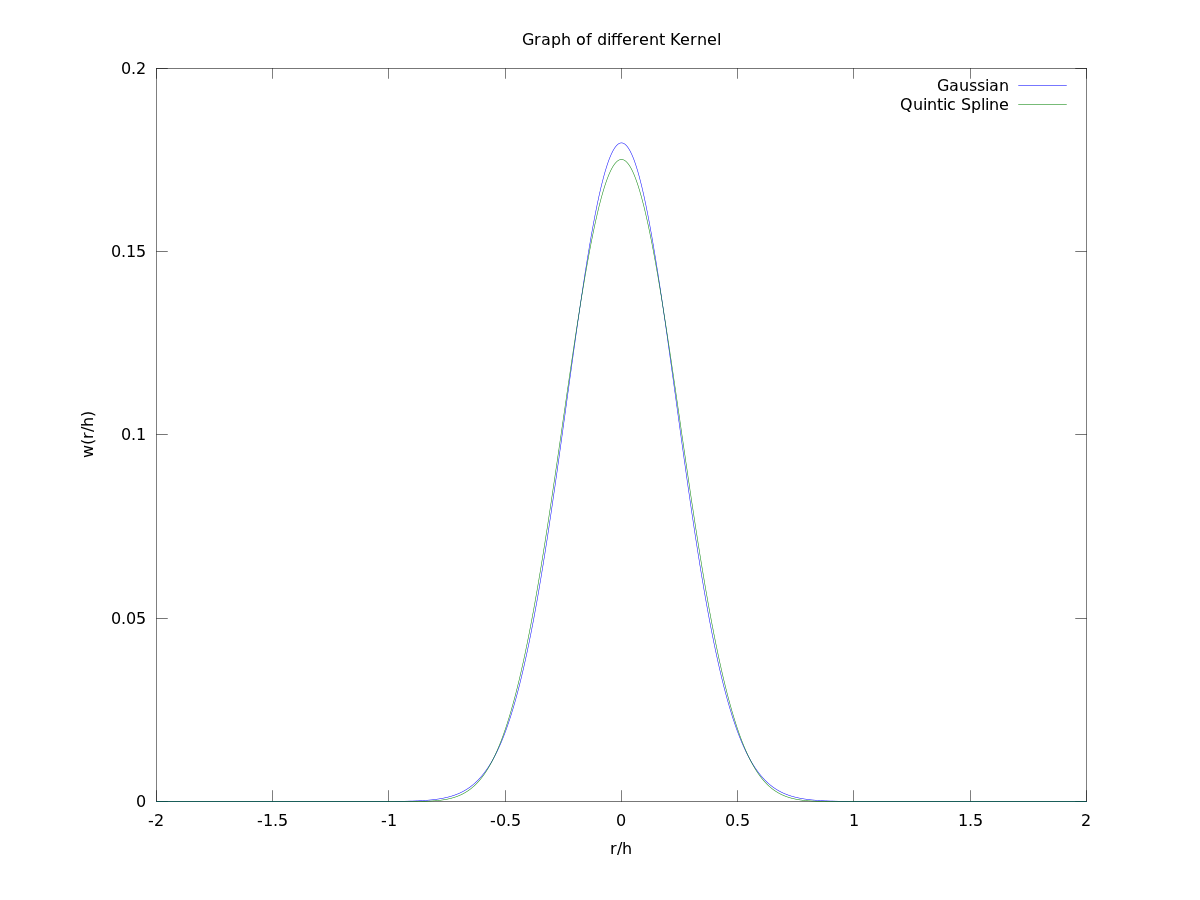
\includegraphics[width=\textwidth]{kernel.png}
\end{frame}

\begin{frame}{Derivée}
 \begin{block}{Intégration par partie}
 \begin{align*}
  <\nabla A(r)>&=\int_{\Omega} \nabla A(r')w_{h}(r-r')dr'+O(h^2)\\
  &=-\int_{\Omega} A(r')\nabla w_{h}(r-r')dr'+O(h^2)
 \end{align*}
\end{block}
\begin{block}{Discretisation}
\begin{equation*}
 \nabla A(r_a)=\sum_{b}A_b\frac{m_b}{\rho_b}\nabla_a w_{h}(r_a-r_b)
 \end{equation*}
\end{block}
\begin{block}{Variante}
 \begin{align*}
  \rho\nabla A&=\nabla(\rho A)-A\nabla \rho\\
  \nabla A(r_a)&=\frac{1}{\rho_a}\sum_{b}m_b \left(A_b-A_a\right) \nabla_a w_{h}(r_a-r_b)
 \end{align*}
\begin{align*}
 \nabla A&=\rho\nabla(\frac{A}{\rho})+\frac{1}{\rho}A\nabla \frac{1}{\rho}\\
 \nabla A(r_a)&=\rho_a\sum_{b} m_b\left(\frac{A_b}{\rho_b^2}+\frac{A_a}{\rho_a^2}\right) \nabla_a w_{h}(r_a-r_b)
\end{align*}

\end{block}


\end{frame}

\begin{frame}{Autre derivée}
 \begin{block}{Divergence}
  On obtient les formules pour la divergence de façon similaire que pour le gradient.
 \end{block}

 \begin{block}{Laplacien}
 \begin{equation*}
  \nabla \phi_{i}=\sum_{j}\frac{e_{ij}}{r_{ij}}\left(\phi_{i}-\phi_{j}\right)
  \end{equation*}
 \end{block}

\end{frame}

\begin{frame}{Smoothing function}
 \begin{block}{Definition}
 \begin{equation*}
  \xi(r)=\frac{w(r-r_{i},h)}{\sum_{b} w(r-r_b)}=\frac{w_{i}(r)}{\sigma(r)}
  \end{equation*}
 \end{block}
\begin{block}{Volume}
 \begin{equation*}
  V_{i}=\int \xi_{i}(r) dr=\int \frac{1}{\sigma(r)}w(r-r_i)dr\approx \frac{1}{\sigma_i}
 \end{equation*}

\end{block}
\begin{block}{Moyenne}
 \begin{equation*}
  <A(r)>=\frac{1}{V}\int \xi_{i}(r)A(r)dr\approx \sigma_{i}\int \xi_{i}(r)A(r)dr
 \end{equation*}

\end{block}

\begin{block}{Densitée}
 \begin{equation*}
  \rho=\frac{m}{V}=m\sigma
 \end{equation*}
\end{block}

\begin{block}{Masse initial}
\begin{equation*}
 m=\frac{\rho_0}{\sigma}
\end{equation*}
\end{block}
\end{frame}

\begin{frame}{Derivée en smoothing function}
\begin{block}{Gradient}
 \begin{equation*}
  \nabla A=\sigma_{a}\sum_{b}\left(\frac{1}{\sigma_{a}^2}+\frac{1}{\sigma_{b}^2}\right)\frac{1}{2}\left(A_a+A_b\right)\nabla w
 \end{equation*}

\end{block}

\begin{block}{Laplacien}
\begin{equation*}
 \Delta A=\sigma_{a}\sum_{b}\left(\frac{1}{\sigma_{a}^2}+\frac{1}{\sigma_{b}^2}\right)\frac{A_a-A_b}{r_{ab}}\frac{\partial w}{\partial r_{ab}}
\end{equation*}

\end{block}
\end{frame}

\begin{frame}{Equations de Navier-Stoke}
 
\begin{align*}
\vect{\nabla} \cdot \vect{u}_{\lambda}(t)&=0\\
\rho\frac{d \vect{u}_{\lambda}(t)}{d t}&=-\vect{\nabla} p(\vect{\xi}_{\lambda}(t),t)+\vect{F}(\vect{\xi}_{\lambda}(t),t)+\mu \Delta \vect{u}_{\lambda}(t)
\end{align*}

\begin{block}{Faible compressible}
\begin{align*}
 p&=B\left(\left(\frac{\rho}{\rho_{0}}\right)^\gamma-1\right)\\
 \gamma&=7\\
 B&=\frac{\rho_0 c_s^2}{\gamma}
 \end{align*}
\end{block}

\begin{block}{Exactement incompressible}
 \begin{enumerate}
  \item Projecter la vitesse pour être à divergence nulle.
  \item Obtenir une densité égual à la densité voulue $\rho_0$.
 \end{enumerate}
\begin{equation*}
 \frac{\dot{\rho}}{\rho}=\nabla \cdot v
\end{equation*}

\end{block}

\end{frame}

\begin{frame}{Avantage et defaut}
 \begin{block}{Faiblement compressible}
  \begin{itemize}
   \plusitem Pas de système linéaire à résoudre.
   \moinsitem Convergence depend de l'intégrateur en temps et des paramêtres.
   \moinsitem Le choix des paramêtres depend du problème.
  \end{itemize}

 \end{block}
 
 \begin{block}{Exactement incompressible}
 \begin{itemize}
  \plusitem Divergence nulle exact.
  \moinsitem Système linéaire à résoudre.
  \moinsitem Système linéaire en general pas symétrique ni defini positif.
 \end{itemize}
  
 \end{block}

\end{frame}

\begin{frame}[shrink]{Loi de conservation}
\begin{block}{Quantité de mouvement}
 \begin{align*}
  P&=\sum_{i} m_iv_{i}\\
  \dot{P}&=\sum_{i} m_ia_{i}\\
  &=\sum_{i}m_{i} \left(-\frac{1}{\rho_{i}}\nabla p+\nu \Delta v\right)\\
  \intertext{Antisymetrie}
  &=0
 \end{align*}

\end{block}

\begin{block}{Moment cinétique}
 \begin{align*}
  M&=\sum_{i}x_{i}\times m_{i}v_{i}\\
  \dot{M}&=\sum_{i}\left(v_{i}\times m_{i}v_{i}+x_{i}\times m_{i}a_{i}\right)\\
  &=\sum_{i}x_{i}\times m_{i}\left(-\frac{1}{\rho_{i}}\nabla p+\nu \Delta v\right)\\
  &=\sum_{a,b}\left(x_{a}-x_{b}\right)\times A_{ab}
 \end{align*}

\end{block}

 
\end{frame}

\begin{frame}[shrink]{Algorithm faible incompressible}
\begin{block}{Crée particule initial:}
	\begin{enumerate}
		\item Placer des particules avec position et vitesse initial.
		\item Choisire la masse des particules de sorte que la densité soit bonne.
		\begin{enumerate}
			\item La densité est donnée par:
			\begin{equation*}
			\Sigma_{a}=\sum_{b}w_{ab}
			\end{equation*}
			\item La masse est donné par:
			\begin{equation*}
			m_a=\frac{\rho_{0}}{\Sigma_{a}}
			\end{equation*}
		\end{enumerate}
	\end{enumerate}
\end{block}
\begin{block}{Pour tout pas de temps:}
	\begin{enumerate}
		\item Integrée les équations de Navier-Stoke. Pour chaque étage:
		\begin{enumerate}
			\item Calculez la densité:
			\begin{equation*}
			\Sigma_{a}=\sum_{b}w_{ab}
			\end{equation*}
			\item Calculez la presion:
			\begin{equation*}
			p=B \left[\left(\frac{m_{a}\sigma_{a}}{\rho_{0}}\right)^{\gamma}-1\right]
			\end{equation*}
			\item Calculez l'acceleration:
			\begin{equation*}
			a_a=-\frac{\nabla p}{m_{a}\sigma_{a}}+g+\nu \Delta v_{a}
			\end{equation*}
			\item Aller au prochain pas de temps avec par exemple:
			\begin{align*}
			x^{n+1}_{a}&=x^{n}_{a}+v^{n}_a\Delta t\\
			v^{n+1}_{a}&=v^{n}_{a}+a^{n}_{a}\Delta t
			\end{align*}
		\end{enumerate}
	\end{enumerate}
\end{block}
\end{frame}
 
 \begin{frame}[shrink]{Algorithm incompressible}
\begin{block}{Crée particule initial:}
	\begin{enumerate}
		\item Placer des particules avec position et vitesse initial.
		\item Choisire la masse des particules de sorte que la densité soit bonne.
		\begin{enumerate}
			\item La densité est donnée par:
			\begin{equation*}
			\Sigma_{a}=\sum_{b}w_{ab}
			\end{equation*}
			\item La masse est donné par:
			\begin{equation*}
			m_a=\frac{\rho_{0}}{\Sigma_{a}}
			\end{equation*}
		\end{enumerate}
	\end{enumerate}
\end{block}
\begin{block}{Pour tout pas de temps:}
	\begin{enumerate}
		\item Integrer les équations de Navier-Stokes sans presion.  Pour chaque étage:
		\begin{enumerate}
			\item Calculez la densité:
			\begin{equation*}
			\Sigma_{a}=\sum_{b}w_{ab}
			\end{equation*}
			\item Calculez l'acceleration:
			\begin{equation*}
			a_a=-\frac{\nabla p}{m_{a}\sigma_{a}}+g+\nu \Delta v_{a}
			\end{equation*}
			\item Aller au prochain pas de temps avec par exemple:
			\begin{align*}
			x^{n+1}_{a}&=x^{n}_{a}+v^{n}_a\Delta t\\
			v^{n+1}_{a}&=v^{n}_{a}+a^{n}_{a}\Delta t
			\end{align*}
		\end{enumerate}
		\item Corrigez la vitesse et la position.
		\begin{enumerate}
			\item Calculez la densité:
			\begin{equation*}
			\Sigma_{a}=\sum_{b}w_{ab}
			\end{equation*}
			\item Corrigez la position:
			\begin{enumerate}[<*>]
				\item Resoudre $p$ dans l'équation linéaire:
				\begin{equation*}
				\sum_{b}\left(\frac{1}{\sigma_{a}^2}+\frac{1}{\sigma_{b}^2}\right)\frac{\partial w}{\partial r_{ab}}\frac{1}{r_{ab}}\frac{p_a-p_b}{m_a\sigma_{a}-m_{b}\sigma_{b}} =\frac{1}{2}\frac{\rho^{0}-m_{a}\sigma_{a}}{\rho_{0}\sigma_{a}}
				\end{equation*}
				\item Correction à:
				\begin{equation*}
				x^{n+1}_{a}=x^{*n+1}_{a}-\frac{1}{m_a}\sum_{b}\left(\frac{1}{\sigma_{a}^2}+\frac{1}{\sigma_{b}^2}\right)\frac{\partial w}{\partial r_{ab}}\frac{\rho_{a}p_{b}+\rho_{b}p_{a}}{\rho_a+\rho_b}e_{ab}
				\end{equation*}
				\item Calculez la densité:
				\begin{equation*}
				\Sigma_{a}=\sum_{b}w_{ab}
				\end{equation*}
			\end{enumerate}
			\item Corrigez la vitesse:
			\begin{enumerate}[<*>]
				\item Resoudre $p$ dans l'équation linéaire:
				\begin{equation*}
				\sum_{b}\left(\frac{1}{\sigma_{a}^2}+\frac{1}{\sigma_{b}^2}\right)\frac{\partial w}{\partial r_{ab}}\frac{1}{r_{ab}}\frac{p_a-p_b}{m_a\sigma_{a}-m_{b}\sigma_{b}} =\frac{1}{4}\sum_{b}\left(\frac{1}{\sigma_{a}^2}+\frac{1}{\sigma_{b}^2}\right)\frac{\partial w}{\partial r_{ab}}\left(v_{a}+v_b\right)\cdot e_{ab}
				\end{equation*}
				\item Corrigez la vitesse:
				\begin{equation*}
				v^{n+1}_{a}=v^{*n+1}_{a}-\frac{1}{m_a}\sum_{b}\left(\frac{1}{\sigma_{a}^2}+\frac{1}{\sigma_{b}^2}\right)\frac{\partial w}{\partial r_{ab}}\frac{\rho_{a}p_{b}+\rho_{b}p_{a}}{\rho_a+\rho_b}e_{ab}
				\end{equation*}
			\end{enumerate}
		\end{enumerate}
	\end{enumerate}
\end{block}
 \end{frame}


\begin{frame}{Avantage de SPH et MAC}
 
 \begin{block}{SPH}
  \begin{itemize}
   \plusitem Terme de convection exact.
   \moinsitem Correction de presion plus dure à faire exactement.
   \plusitem Loi de conservation interessante.
   \moinsitem Justification et preuve de convergence plus dure.
   \moinsitem Système linéaire difficil a résoudre.
   \moinsitem Plus de voisin à traiter.
  \end{itemize}

 \end{block}

 \begin{block}{MAC}
  \begin{itemize}
   \plusitem Methode de discretisation bien connu.
   \plusitem Système linéaire facil a résoudre.
   \moinsitem Terme convectif plus dure.
   \plusitem Moins de voisin à traiter.
  \end{itemize}

 \end{block}

 
\end{frame}


\end{document}


